\begin{center}
  \textbf{ВВЕДЕНИЕ}
\end{center}
\addcontentsline{toc}{chapter}{ВВЕДЕНИЕ}

В задачах комбинаторной оптимизации часто нужно найти решение, которое удовлетворяет заданным условиям и при этом требует минимальных затрат времени и ресурсов. Одной из таких классических задач является задача коммивояжёра. Она заключается в поиске самого короткого маршрута, который проходит через все указанные города ровно один раз и возвращается в начальную точку.

Для её решения используют разные подходы, такие как алгоритм полного перебора и метод, основанный на муравьином алгоритме.

Алгоритм полного перебора находит точное решение, проверяя все возможные маршруты и выбирая среди них самый короткий. Однако этот метод ресурсоёмкий, при условии, если количество городов сильно возрастает.

Метод, основанный на муравьином алгоритме, основывается на наблюдении за поведением реальных муравьёв. В поисках пищи они оставляют на своём пути феромоны, которые привлекают других муравьёв, помогая им выбрать кратчайший маршрут. Если на пути встречается препятствие, муравьи ищут обходные пути. Те из них, кто случайно выбирает более короткий маршрут, двигаются быстрее и оставляют больше феромонов, таким образом привлекая остальных. Этот метод позволяет быстро получать решения, что делает его эффективным для практического применения.



Целью данной лабораторной работы является освоение особенностей и оценка эффективности двух методов решения задачи коммивояжёра: муравьиного алгоритма и алгоритма полного перебора.

Для достижения поставленной цели необходимо выполнить следующие задачи:
\begin{itemize}
  \item исследовать особенности задачи коммивояжёра и её применения;
  \item рассмотреть и реализовать алгоритм полного перебора;
  \item рассмотреть и реализовать алгоритм муравьиного алгоритма;
  \item провести исследование производительности и эффективности реализованных алгоритмов при различных входных данных;
  \item сформулировать и представить результаты в отчёте о проведённой лабораторной работе.
\end{itemize}

\newpage

\aasection{Аналитическая часть}{sec:algorithm}

\section{Задача Коммивояжёра}

Задача коммивояжёра заключается в нахождении кратчайшего маршрута, который проходит через все заданные города, посещая каждый из них ровно один раз, и возвращается в исходную точку~\cite{shtovba_ants}. Эта задача может быть рассмотрена как поиск минимального пути в полном графе, где вершины представляют города, а рёбра --- расстояния между ними.

Необходимо выбрать порядок посещения городов так, чтобы суммарное расстояние было минимальным. Задача состоит в нахождении данного порядка с учётом расстояний между городами.

\section{Метод полного перебора}
Метод полного перебора заключается в том, что исследуются все возможные маршруты, и выбирается наиболее оптимальный. Данный алгоритм гарантирует нахождение точного решения задачи.

\begin{itemize}
  \item \textbf{Преимущество:} метод гарантирует нахождение наилучшего решения задачи коммивояжёра, так как перебираются все возможные варианты маршрутов.
  \item \textbf{Недостаток:} сложность метода составляет $O(n!)$, что приводит к экспоненциальному росту времени вычислений с увеличением числа городов.
\end{itemize}

Таким образом, несмотря на то, что метод полного перебора даёт точное решение, его высокая вычислительная сложность ограничивает его использование для задач с большим числом городов.

\section{Метод, основанный на муравьином алгоритме}
Основная идея муравьиного алгоритма заключается в моделировании поведения муравьиной колонии, которая решает задачу коммивояжёра в течение $t_{\text{max}}$ суток. Каждый муравей действует автономно, но его поведение влияет на всю колонию через следы феромонов, оставляемые на пройденном пути~\cite{ulyanov_algorithms}. Эти следы служат сигналом для других муравьёв, направляя их по наиболее выгодным маршрутам. Такое коллективное поведение помогает колонии находить кратчайшие пути и адаптироваться к изменяющимся условиям окружающей среды.

Процесс решения задачи коммивояжёра с использованием муравьиного алгоритма включает следующие этапы:
\begin{enumerate}
  \item[---] утром муравьи выходят из муравейника и распределяются по городам;
  \item[---] в дневной фазе каждый муравей формирует полный маршрут;
  \item[---] к закату муравьи возвращаются в муравейник, где обновляется наилучшие результаты и длина лучшего найденного маршрута $L_{\text{best}}$;
  \item[---] в ночной фазе обновляется матрица феромонов.
\end{enumerate}

Каждый муравей обладает тремя свойствами:
\begin{itemize}
  \item[---] \textbf{зрение} --- муравей $k$ в городе $i$ оценивает привлекательность $\eta_{ij}$ дуги $i-j$ по формуле:
  \begin{equation}
      \eta_{ij} = \frac{1}{D_{ij}},
  \end{equation}
  где $D_{ij}$ — метка дуги; $D$ --- матрица смежности графа.
  
  \item[---] \textbf{память} --- муравей запоминает посещённые города в день $t$ в кортеж $J_k(t)$.
  
  \item[---] \textbf{обоняние} --- муравей чует концентрацию феромонов $\tau_{ij}(t)$ на дуге $i-j$ в день $t$.
  \begin{itemize}
      \item ячейки матрицы феромонов $\tau_{ij}$ инициализируются константой;
      \item значения $\tau_{ij}$ не обновляются в фазу дня.
  \end{itemize}
\end{itemize}

Находясь в городе $i$, муравей $k$ выбирает следующий город $j$ с вероятностью, вычисляемой по формуле \eqref{eq:prob}:

\begin{equation}
\label{eq:prob}
P_{ij, k}(t) = 
\begin{cases}
  0, &\text{если $j \in J_k(t)$}, \\
  {\displaystyle\frac {\eta_{ij}^{\alpha }\tau_{ij}(t)^{\beta }}{
      \displaystyle\sum_{q \notin J_k(t)} (\eta_{iq}^{\alpha}\tau_{iq}^{\beta })}}, &\text{иначе}.
\end{cases}
\end{equation}

В формуле \eqref{eq:prob}:
\begin{itemize}
  \item $\alpha$ и $\beta$ --- коэффициенты жадности и стадности соответственно, причём $\alpha + \beta = 1$:
  \begin{itemize}
      \item при $\alpha = 0$ и $\beta = 1$ поведение полностью стадное;
      \item при $\alpha = 1$ и $\beta = 0$ поведение полностью жадное.
  \end{itemize}
\end{itemize}

Обновление концентрации феромона $\tau_{ij}$ происходит ночью по формуле \eqref{eq:upd}:

\begin{equation}
\label{eq:upd}
\tau_{ij}(t+1) = \tau_{ij}(t) \cdot (1-p) + \Delta\tau_{ij}(t),
\end{equation}
где $p$ --- коэффициент испарения $(p \in (0, 1))$. 

Изменение концентрации феромона на завтра $\Delta\tau_{ij}(t)$ определяется формулой \eqref{eq:chn}:

\begin{equation}
\label{eq:chn}
\Delta\tau_{ij}(t) = \sum_{k=1}^{N} \Delta\tau_{ij, k}(t),
\end{equation}
где $N$ --- количество муравьёв. 

Величина $\Delta\tau_{ij, k}(t)$ вычисляется по формуле \eqref{eq:chn2}:

\begin{equation}
  \label{eq:chn2}
  \Delta\tau_{ij, k}(t) = 
  \begin{cases} 
    0, & \text{если муравей $k$ в день $t$ не использовал дугу}, \\ 
    \frac{Q}{L_k(t)}, & \text{иначе}.
  \end{cases}
\end{equation}

В формуле \eqref{eq:chn2} $Q$ --- дневная квота феромона одного муравья, $L_k(t)$ --- длина маршрута муравья $k$ в день $t$. Значение $Q$ подбирается на тестовом графе следующим образом:

\begin{itemize}
  \item на тестовом графе запускаются расчёты с различными значениями $Q$;
  \item оценивается качество найденных маршрутов при разных значениях $Q$;
  \item выбирается значение $Q$, обеспечивающее хорошие результаты при минимальном количестве итераций.
\end{itemize}

После выбора оптимального значения $Q$ оно вручную задаётся в программе для проведения окончательных расчётов.

Если значение $\tau_{ij}(t)$ становится меньше минимального значения $\tau_{\text{min}}$, оно откатывается к $\tau_{\text{min}}$.

Модификация с элитными муравьями усиливает феромоны на дугах наилучших маршрутов. В этом случае формула \eqref{eq:chn} принимает вид:

\begin{equation}
\Delta\tau_{ij}(t) = \sum_{k=1}^{N} \Delta\tau_{ij, k}(t) + \Delta\tau_{\text{элит}}(t),
\end{equation}
где 
\begin{equation}
\Delta\tau_{\text{элит}}(t) = 
\begin{cases}
  0, & \text{если дуга $i-j$ не принадлежит маршруту $L_{\text{best}}$}, \\
  \frac{Q}{L_{\text{best}}}, & \text{иначе}.
\end{cases}
\end{equation}


\section*{Вывод}
В данном разделе рассмотрены алгоритмы решения задачи коммивояжёра: метод полного перебора и метод, основанный на муравьином алгоритме. Метод полного перебора обеспечивает нахождение оптимального пути, но его применение ограничено высокой вычислительной сложностью. Метод, основанный на муравьином алгоритме, хотя и позволяет быстро находить решения, обеспечивает более быстрое решение, что делает его предпочтительным для задач с большим числом городов.


\aasection{Конструкторская часть}

В данном разделе представлены описания алгоритмов решения задачи коммивояжёра: метод полного перебора и метод, основанный на муравьином алгоритме. Описана структура программного обеспечения, а также алгоритмы, реализующие данные методы, и их взаимодействие с пользователем.

\section{Описание структуры ПО}

На вход программного продукта подаётся взвешенный граф в виде матрицы смежности. Метод, основанный на муравьином алгоритме также принимает начальные значения феромонов, максимальное количество итераций, коэффициенты $\alpha$ и $\beta$, а также коэффициент испарений. Программа позволяет пользователю выбрать один из двух алгоритмов: метод полного перебора или метод, основанный на муравьином алгоритме.

\section{Описание алгоритмов}

В программном продукте реализованы два алгоритма для решения задачи коммивояжёра.

\begin{enumerate}
  \item[---] \textbf{Метод полного перебора}, который анализирует все возможные маршруты и выбирает оптимальный. Данный метод гарантирует нахождение наилучшего решения, но имеет высокую вычислительную сложность.
  \item[---] \textbf{Метод, основанный на муравьином алгоритме}, который использует вероятностный подход для нахождения решения. Данный метод позволяет быстро находить решения, но не всегда гарантирует оптимальный путь.
\end{enumerate}

Метод, основанный на муравьином алгоритме реализуется с учётом коэффициентов жадности $\alpha$ и стадности $\beta$, что влияет на поведение муравьёв при выборе путей. Алгоритм работает итеративно, обновляя значения феромонов и выбирая пути с учётом вероятностного распределения.

\section{Алгоритм взаимодействия с пользователем}

Программа взаимодействует с пользователем через консоль. Процесс работы с программой следующий.

Пользователь выбирает режим ввода данных:
\begin{itemize}
  \item из файла;
  \item из консоли.
\end{itemize}

  \item[---] В случае выбора ввода из файла, программа запрашивает имя файла и загружает данные о графе (количество городов, количество дорог, данные о дорогах).
  \item[---] В случае выбора консольного ввода, программа запрашивает количество городов и количество дорог и информацию о каждой дороге (стартовый и конечный города, вес дороги).
  \item[---] Далее пользователю предлагается выбрать алгоритм для решения задачи:
  \begin{itemize}
      \item метод, основанный на муравьином алгоритме (Ant Colony Optimization);
      \item метод полного перебора (Brute Force).
  \end{itemize}
  \item[---] Если выбран метод, основанный на муравьином алгоритме, программа запрашивает дополнительные параметры:
  \begin{itemize}
      \item количество итераций;
      \item количество муравьёв в каждом городе;
      \item количество элитных муравьёв;
      \item коэффициент испарения феромонов;
      \item значения феромонов для общего пути и для элитных муравьёв;
      \item коэффициенты для феромонов и веса пути.
  \end{itemize}
  \item[---] Если выбран метод полного перебора, программа сразу выполняет поиск наилучшего пути, анализируя все возможные маршруты.
  \item[---] В обоих случаях программа выводит наилучший найденный путь, его длину, порядок посещённых городов и время выполнения алгоритма.
\end{itemize}

На рисунках~\ref{fig:brute} и~\ref{fig:ant_alg} приведены схемы реализации алгоритмов полного перебора и муравьиного алгоритма.

\clearpage

\begin{figure}[H]
  \centering
  \hspace{1cm} 
  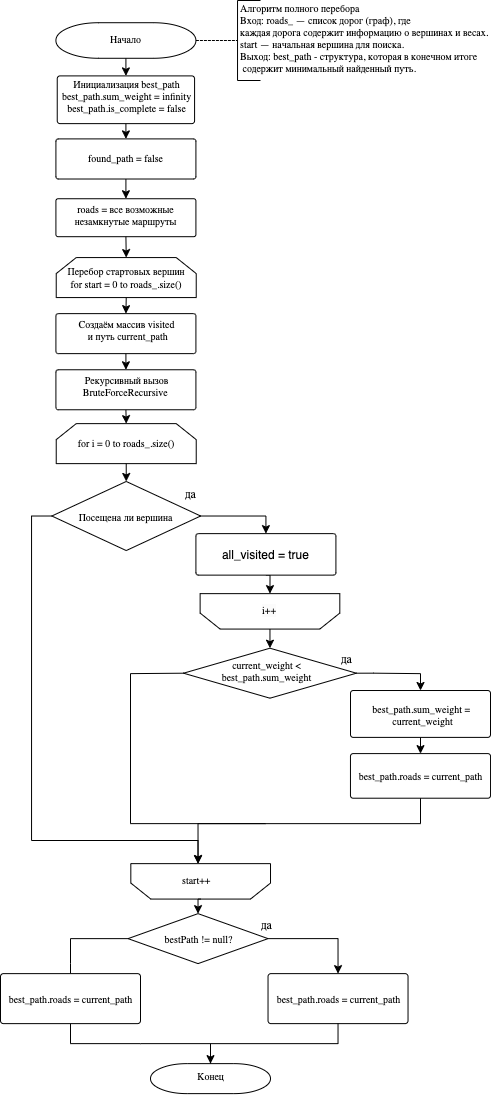
\includegraphics[width=0.6\textwidth]{inc/img/123.drawio.png}
  \caption{Схема алгоритма полного перебора}
  \label{fig:brute}
\end{figure}

\begin{figure}[H]
  \centering
  \hspace{1cm} 
  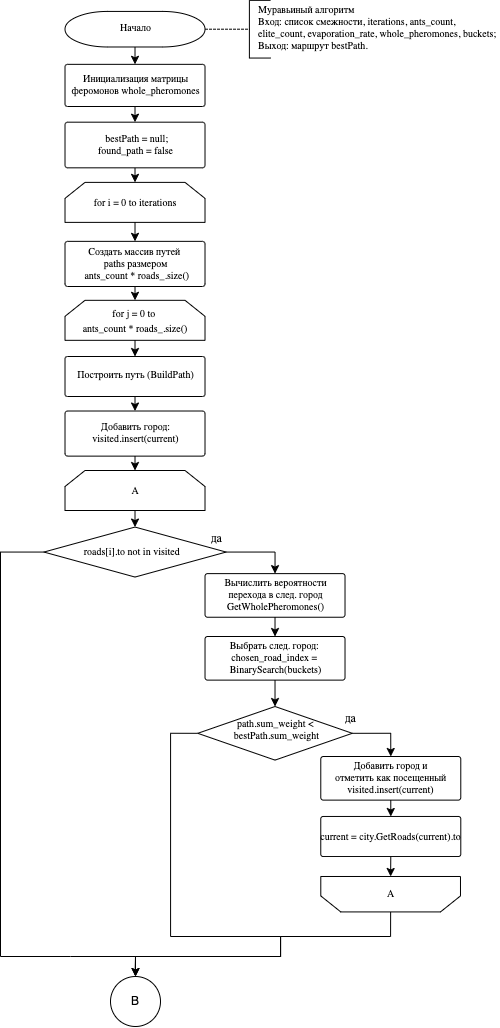
\includegraphics[width=0.7\textwidth]{inc/img/111.drawio.png}
  \caption{Схема муравьиного алгоритма (начало)}
  \label{fig:ant_alg}
\end{figure}

\begin{figure}[H]
  \centering
  \hspace{1cm} 
  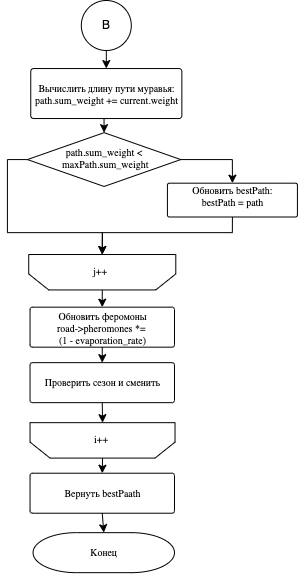
\includegraphics[width=0.5\textwidth]{inc/img/222.drawio.png}
  \caption{Схема муравьиного алгоритма (продолжение)}
  \label{fig:ant_alg2}
\end{figure}


\newpage
\aasection{Технологическая часть}{sec:tec}
В данном разделе приведены данные о выбранном языке программирования и реализации алгоритмов поиска.

\section{Средства реализации}
Для реализации алгоритмов поиска, проведения замеров времени и обработки данных в данной работе используется язык программирования \texttt{C++}~\cite{stroustrup_cpp}. Язык предоставляет мощные инструменты для работы с массивами, а также позволяет эффективно управлять временем выполнения с помощью различных библиотек.


\section{Реализация алгоритмов}

В листинге~\ref{lst:choose_road} представлена функция \texttt{ChooseRoad} для выбора дороги в муравьином алгоритме.


\begin{center}
\captionsetup{justification=raggedright,singlelinecheck=off}
\captionof{lstlisting}{Метод выбора дороги для муравья}
\label{lst:choose_road}
\begin{framed}
\begin{lstlisting}[language=C++]
size_t Ant::ChooseRoad(const std::vector<Road>& roads, double ph_pow, double weight_pow,
                     std::unordered_set<size_t>& visited) {
std::vector<size_t> roads_indices;
for (size_t i = 0; i < roads.size(); ++i) {
  if (visited.find(roads[i].to) == visited.end()) {
    roads_indices.push_back(i);
  }
}
if (roads_indices.empty()) {
  return roads.size();
}
double whole_pheromones = GetWholePheromones(roads_indices, roads, ph_pow, weight_pow);
std::vector<double> buckets(roads_indices.size() + 1);
buckets[0] = 0;
for (size_t i = 1; i < buckets.size(); ++i) {
  buckets[i] = buckets[i - 1] + GetCoefficient(roads[roads_indices[i - 1]], ph_pow, weight_pow);
}
for (int i = 0; i < buckets.size(); ++i) {
  buckets[i] /= whole_pheromones; }
std::random_device rd;
std::mt19937 gen(rd());
std::uniform_real_distribution<> dis(0, buckets.back());
double value = dis(gen);
return roads_indices[BinarySearch(buckets, value) - 1];
}
\end{lstlisting}
\end{framed}
\end{center}


В листинге~\ref{lst:build_path} представлена функция \texttt{BuildPath} для построения пути для муравья.

\begin{center}
\captionsetup{justification=raggedright,singlelinecheck=off}
\captionof{lstlisting}{Метод построения пути для муравья}
\label{lst:build_path}
\begin{framed}
\begin{lstlisting}[language=C++]
Path Ant::BuildPath(City& city, size_t start, double ph_pow, double weight_pow) {
Path path;
path.is_complete = false;
size_t current = start;
std::unordered_set<size_t> visited;
visited.insert(current);
path.sum_weight = 0;
while (visited.size() < city.GetSize()) {
  size_t chosen_road_index = ChooseRoad(city.GetRoads(current), ph_pow, weight_pow, visited);
  if (chosen_road_index == city.GetRoads(current).size()) {
    return path; }
  path.roads.push_back(
      &city.GetRoads(current)[chosen_road_index]);
  path.sum_weight += city.GetRoads(current)[chosen_road_index].weight;
  current = city.GetRoads(current)[chosen_road_index].to;
  visited.insert(current); }
path.is_complete = true;
path.start = start;
return path; }
\end{lstlisting}
\end{framed}
\end{center}

В листинге~\ref{lst:crowl} представлена функция \texttt{Crowl} для муравьиного алгоритма.

\begin{center}
\captionsetup{justification=raggedright,singlelinecheck=off}
\captionof{lstlisting}{Метод муравьиного алгоритма для поиска пути}
\label{lst:crowl}
\begin{framed}
\begin{lstlisting}[language=C++]
Path City::Crowl(size_t iterations, size_t ants_count, size_t elite_count, double evaporation_rate,
               double common_pheromones, double elite_pheromones, double ph_pow, double weight_pow) {
Path best_path;
bool found_path = false;
for (size_t i = 0; i < iterations; ++i) {
  std::vector<Path> paths(ants_count * roads_.size());
  for (size_t j = 0; j < ants_count * roads_.size(); ++j) {
    size_t start = j % roads_.size();
    paths[j] = Ant().BuildPath(*this, start, ph_pow, weight_pow);
  }
  for (auto& path : paths) {
    for (auto& road : path.roads) {
      road->pheromones *= (1 - evaporation_rate);
    }
  }
  std::sort(paths.begin(), paths.end(), [](const Path& a, const Path& b) {
    if (a.is_complete && !b.is_complete) {
      return true;
    }
    if (!a.is_complete && b.is_complete) {
      return false;
    }
    return a.sum_weight < b.sum_weight;
  });
  for (size_t j = 0; j < elite_count; ++j) {
    if (!paths[j].is_complete) {
      continue;
    }
    for (auto& road : paths[j].roads) {
      road->elite_visited = true;
    }
  }
  for (size_t j = elite_count; j < paths.size(); ++j) {
    if (!paths[j].is_complete) {
      continue;
    }
    for (auto& road : paths[j].roads) {
      road->visited = true;
    }
  }
  for (auto& path : paths) {
    for (auto& road : path.roads) {
      if (road->elite_visited) {
        road->pheromones += elite_pheromones;
      } else if (road->visited) {
        road->pheromones += common_pheromones;
      }
      road->elite_visited = false;
      road->visited = false;
    }
  }
  if (paths[0].is_complete && (!found_path || paths[0].sum_weight < best_path.sum_weight)) {
    best_path = paths[0];
    found_path = true;
  }
}
return best_path;
}
\end{lstlisting}
\end{framed}
\end{center}

В листинге~\ref{lst:brute_force} представлена функция \texttt{BruteForce} для решения задачи коммивояжёра методом полного перебора.

\begin{center}
\captionsetup{justification=raggedright,singlelinecheck=off}
\captionof{lstlisting}{Метод полного перебора для решения задачи коммивояжёра}
\label{lst:brute_force}
\begin{framed}
\begin{lstlisting}[language=C++]
Path City::BruteForce() {
Path best_path;
best_path.sum_weight = std::numeric_limits<double>::infinity();
best_path.is_complete = false;
bool found_path = false;
for (size_t start = 0; start < roads_.size(); ++start) {
  std::vector<size_t> cities(roads_.size());
  for (size_t i = 0; i < cities.size(); ++i) {
    cities[i] = i;}
  cities.erase(std::find(cities.begin(), cities.end(), start));
  do {
    Path path;
    path.is_complete = true;
    path.sum_weight = 0;
    size_t current = start;
    for (size_t i = 0; i < cities.size(); ++i) {
      size_t next = cities[i];
      auto it = std::find_if(roads_[current].begin(), roads_[current].end(),
                             [next](const Road& r) { return r.to == next; });
      if (it != roads_[current].end()) {
        path.roads.push_back(&(*it));
        path.sum_weight += it->weight;
        current = next;
      } else {
        path.is_complete = false;
        break;
      }
    }
    if (path.is_complete && path.sum_weight < best_path.sum_weight) {
      best_path = path;
    }
  } while (std::next_permutation(cities.begin(), cities.end())); }
return best_path; }
\end{lstlisting}
\end{framed}
\end{center}


\section{Тестирование результатов поиска пути}

В таблице~\ref{tbl:functional_test} приведены результаты функционального тестирования для алгоритмов поиска пути, использующих полный перебор и метод, основанный на муравьином алгоритме. Оба метода тестировались на одинаковых входных данных для проверки корректности их работы. Основное различие в подходе: полный перебор гарантирует оптимальное решение, а муравьиный алгоритм предоставляет решение за меньшее время.

\begin{longtable}{|p{.05\textwidth - 2\tabcolsep}|p{.33\textwidth - 2\tabcolsep}|p{.33\textwidth - 2\tabcolsep}|p{.19\textwidth - 2\tabcolsep}|}
  \caption{Функциональные тесты алгоритмов поиска пути}\label{tbl:functional_test} \\\hline
  № теста & Входные данные & Ожидаемый результат & Результат теста \\\hline
  \endfirsthead
  \caption{Функциональные тесты алгоритмов поиска пути (продолжение)} \\\hline
  № теста & Входные данные & Ожидаемый результат & Результат теста \\\hline
  \endhead
  \endfoot
  1 & Матрица смежности: 
  \(\begin{pmatrix}
  0 & 1 & 2 & 3 & 4 & 5 \\
  1 & 0 & 6 & 7 & 8 & 9 \\
  2 & 6 & 0 & 10 & 11 & 12 \\
  3 & 7 & 10 & 0 & 13 & 14 \\
  4 & 8 & 11 & 13 & 0 & 15 \\
  5 & 9 & 12 & 14 & 15 & 0
  \end{pmatrix}\) &
  3.5, (0, 3, 1, 6, 5, 2, 4) &
  Успех (Решение найдено с использованием метода, основанного на муравьином алгоритме) \\\hline
  2 & Матрица смежности:
  \(\begin{pmatrix}
  0 & 1 & 2 & 3 & 4 & 5 \\
  1 & 0 & 6 & 7 & 8 & 9 \\
  2 & 6 & 0 & 10 & 11 & 12 \\
  3 & 7 & 10 & 0 & 13 & 14 \\
  4 & 8 & 11 & 13 & 0 & 15 \\
  5 & 9 & 12 & 14 & 15 & 0
  \end{pmatrix}\) &
  3.5, (0, 3, 1, 6, 5, 2, 4) &
  Успех (Решение найдено с использованием метода полного перебора) \\\hline
\end{longtable}

\section{Результаты исследования}

Тестирование подтвердило корректность асимптотической сложности алгоритмов:

\begin{itemize}
  \item метод на основе муравьиного алгоритма имеет сложность \(O(I \cdot A \cdot (V + E))\), где \(I\) --- количество итераций, \(A\) --- количество муравьёв, \(V\) --- число вершин, \(E\) --- число рёбер.
  \item алгоритм полного перебора имеет сложность \(O(V!)\), так как количество перестановок вершин растёт факториально.
\end{itemize}

Измерение времени выполнения относится не к самим алгоритмам, а к их программной реализации, которая зависит от платформы, кода и условий тестирования. На рисунке~\ref{fig:comp} представлено сравнение времени работы двух методов в зависимости от размера графа. Это сравнение показывает практическую эффективность программной реализации для каждого метода.

Основные различия тестов для двух методов:
\begin{itemize}
  \item метод полного перебора гарантирует нахождение оптимального решения, но требует больше времени для больших графов;
  \item метод на основе муравьиного алгоритма быстрее, но может предоставлять решение, что подходит для задач, где допустима погрешность.
\end{itemize}


\section{Пример работы программы} \label{sec:demod}
На рисунке~\ref{img:ant} представлена демонстрация работы программы.
\begin{figure}[h]
  \centering
  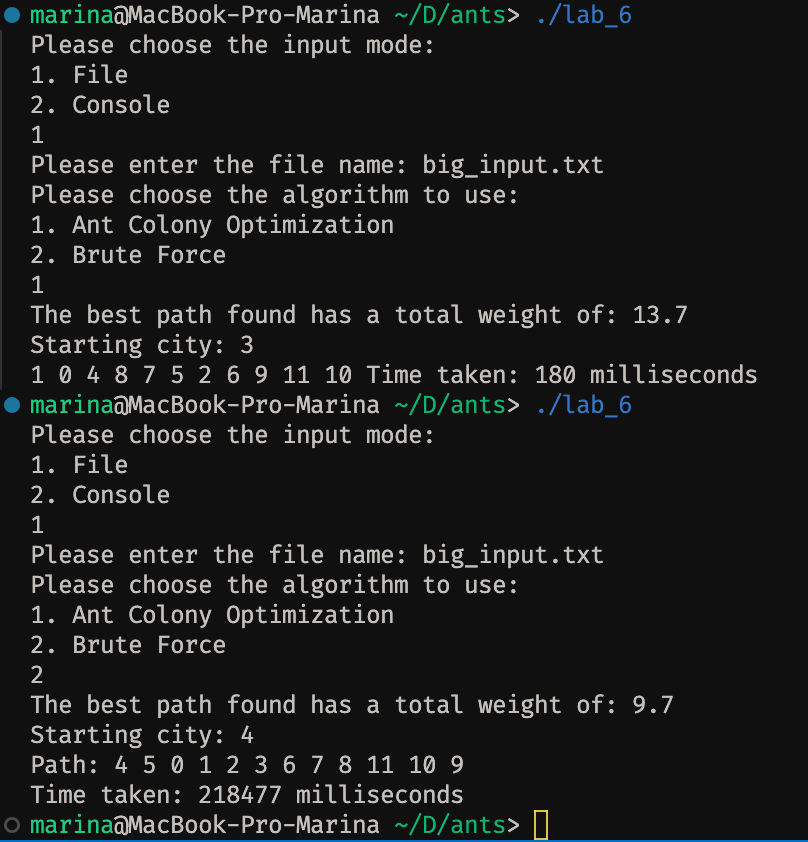
\includegraphics[width=0.6\textwidth]{inc/img/ant.png}  % уменьшаем размер изображения до 80% от ширины текста
  \caption{Демонстрация работы программы}
  \label{img:ant}  % метка рисунка
\end{figure}

\section*{Вывод}
В данном разделе представлены результаты тестирования алгоритмов поиска пути. Все тесты пройдены успешно, фактические результаты совпадают с ожидаемыми.

\aasection{Исследовательская часть}{sec:study}
В данном разделе представлены результаты исследования эффективности работы алгоритмов по времени выполнения, основанной на критерии временных затрат.

\section{Технические характеристики}
Технические характеристики компьютера, на котором проводились замеры времени:

\begin{itemize} 
  \item[--] операционная система: macOS Monterey;
  \item[--] оперативная память: 8 ГБ;
  \item[--] процессор: Quad-Core Intel Core i5;
\end{itemize}

\section{Результаты исследования}
В таблице~\ref{tbl:time_measurements} представлено время выполнения алгоритмов Ant Colony Optimization и Brute Force для графов с различным количеством вершин, измеренное в миллисекундах.

Для каждого графа и каждой тройки параметров муравьиного алгоритма (\(I\) --- число итераций, \(A\) --- количество муравьёв, \(\rho\) --- коэффициент испарения феромонов) было выполнено 50 измерений времени работы для каждого из алгоритмов. Результаты измерений усреднялись. Время замерялось с помощью встроенной функции времени в языке C++. 

Алгоритм полного перебора был значительно медленнее, чем метод, основанный на муравьином алгоритме, особенно при увеличении количества вершин в графе.

\begin{table}[h]
  \begin{center}
      \begin{threeparttable}
          \captionsetup{justification=raggedright,singlelinecheck=off}
          \caption{Время выполнения алгоритмов в зависимости от входных данных (в миллисекундах)}
          \label{tbl:time_measurements}
          \small
          \begin{tabular}{|r|r|r|}
              \hline
              Количество вершин & Алгоритм полного перебора & Муравьиный алгоритм \\
              \hline
              3 & 0 & 0 \\
              \hline
              4 & 0 & 1 \\
              \hline
              5 & 1 & 7 \\
              \hline
              6 & 2 & 7 \\
              \hline
              7 & 2 & 17 \\
              \hline
              9 & 53 & 20 \\
              \hline
              10 & 200 & 31 \\
              \hline
              11 & 913 & 32 \\
              \hline
          \end{tabular}
      \end{threeparttable}
  \end{center}
\end{table}

На рисунке~\ref{fig:comp} показано, как изменяется время выполнения алгоритмов в зависимости от количества вершин для метода, основанном на муравьином алгоритме и метода полного перебора.

\begin{figure}[h!]
  \centering
  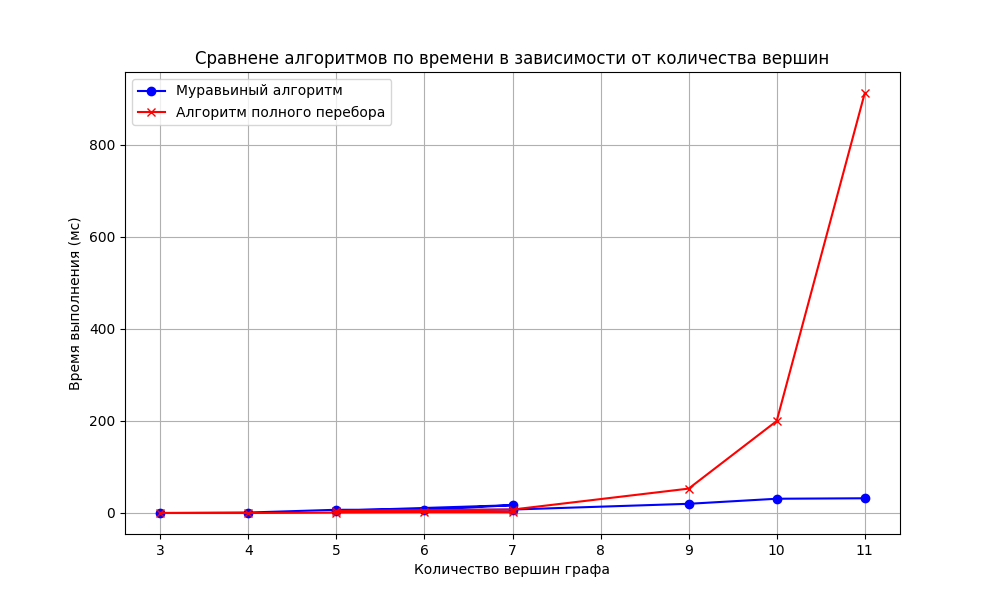
\includegraphics[scale=0.7]{inc/img/comp.png}
  \caption{Зависимость времени выполнения алгоритмов от количества вершин}
  \label{fig:comp}
\end{figure}
\section{Результаты параметризации}

В ходе параметризации исследовались различные комбинации параметров, таких как количество итераций (\(I\)), количество муравьёв (\(A\)) и коэффициент испарения феромонов (\(\rho\)), с целью оптимизации работы алгоритма. Результаты приведены в таблице, где указаны максимальные, медианные и средние значения отклонений стоимости маршрута от эталонного.

\begin{table}[h]
\centering
\caption{Время выполнения алгоритмов в зависимости от параметров (в миллисекундах)}
\label{tbl:param_results}
\small
\begin{tabular}{|r|r|r|r|r|r|r|r|r|}
\hline
\(\alpha\) & \(\rho\) & \(I\) & max\_t1 & avg\_t1 & med\_t1 & max\_t2 & avg\_t2 & med\_t2 \\
\hline
0.5 & 0.3 & 50 & 3.10 & 0.95 & 0.05 & 6.10 & 5.20 & 6.05 \\
1.0 & 0.3 & 50 & 0.10 & 0.05 & 0.00 & 9.10 & 7.00 & 6.10 \\
1.5 & 0.3 & 50 & 0.00 & 0.00 & 0.00 & 9.10 & 7.60 & 7.55 \\
2.0 & 0.1 & 100 & 1.05 & 0.15 & 0.05 & 6.05 & 4.25 & 4.55 \\
2.5 & 0.1 & 100 & 0.00 & 0.00 & 0.00 & 9.05 & 6.65 & 6.05 \\
1.0 & 0.3 & 100 & 0.00 & 0.00 & 0.00 & 9.05 & 7.55 & 9.05 \\
\hline
\end{tabular}
\end{table}

Результаты параметризации показывают, что метод, основанный на муравьином алгоритме значительно сокращает время работы для небольших графов.

\section*{Вывод}
Результаты исследования показывают значительное различие в времени выполнения между двумя алгоритмами. Метод, основанный на муравьином алгоритме показал значительное сокращение времени выполнения для небольших графов, но с увеличением количества вершин время выполнения увеличивается. Алгоритм полного перебора демонстрирует резкое увеличение времени при росте числа вершин, что делает его менее эффективным для больших графов.

Например, для графа с 5 вершинами время работы муравьиного алгоритма составило 7 миллисекунд, в то время как алгоритм полного перебора потребовал 200 миллисекунд. Для графов с 11 вершинами время работы муравьиного алгоритма всего 32 миллисекунды, тогда как алгоритм полного перебора занял 913 миллисекунд.

Таким образом, метод, основанный на муравьином алгоритме наиболее эффективен для задач с большим количеством вершин, так как его время выполнения значительно ниже по сравнению с алгоритмом полного перебора, который становится менее эффективным при увеличении размера графа.


\clearpage
\aaunnumberedsection{ЗАКЛЮЧЕНИЕ}{sec:outro}

Цель лабораторной работы была достигнута. В ходе выполнения работы решены следующие задачи:

\begin{itemize}
  \item исследованы особенности задачи коммивояжёра и её применения, включая трудности нахождения оптимального пути для большого числа городов;
  \item рассмотрен и реализован алгоритм полного перебора, который обеспечивает точное решение, но имеет высокие вычислительные затраты при увеличении количества городов;
  \item рассмотрен и реализован метод, основанный на муравьином алгоритме, который является эвристическим методом, способным находить решения с меньшими вычислительными затратами;
  \item проведено исследование производительности и эффективности реализованных алгоритмов при различных входных данных;
  \item сформулированы и представлены результаты в отчёте о проведённой лабораторной работе.
\end{itemize}

Исследования показали, что метод, основанный на муравьином алгоритме значительно быстрее, особенно при решении задач с большим числом вершин. В отличие от алгоритма полного перебора, который даёт точные результаты, но его время выполнения резко увеличивается с ростом количества вершин, что делает его трудным для использования при решении больших задач. Метод, основанный на муравьином алгоритме, в свою очередь, сохраняет хорошую эффективность и существенно ускоряет поиск решения, оставаясь эффективным даже для крупных графов.

Таким образом, для задач, где важна скорость нахождения решения, особенно при большом числе вершин, метод, основанный на муравьином алгоритме является предпочтительным. Алгоритм полного перебора лучше подходит для небольших и средних графов, где важна точность результата.